\chapter{Teoria}
\label{cha:wstep}

Aby móc zagłębić się w temat, należy najpierw wyjaśnić, jak działają poszczególne rozwiązania wykorzystywane w procesorach oraz jak dane są pobierane przez procesor.

\section{Przetwarzanie potokowe (ang. \textit{pipelining})}

Wykonywanie instrukcji przez procesor składa się z kilku etapów. W zależności od procesora może być ich różna ilość. Etapy, które musi wykonać procesor, to:

\begin{itemize}
	\item Pobieranie instrukcji (ang. \textit{IF -- instruction fetch}),
	\item Dekodowanie instrukcji (ang. \textit{ID -- instruction decode}),
	\item Wykonywanie instrukcji (ang. \textit{EX -- execute}),
	\item Zapisywanie rezultatu (ang. \textit{WB -- writeback}).
\end{itemize}


\begin{figure}[!h]
	\centering
	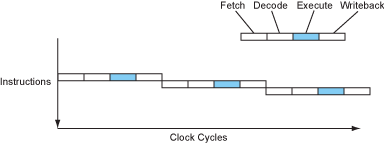
\includegraphics[width=0.7\textwidth]{images/sequential2}
	\caption{Przepływ wykonywania instrukcji przez procesor sekwencyjny \cite{ModernMicroprocessors90MinGuide}.}
\end{figure}

Nowoczesne procesory, zamiast przetwarzać instrukcje sekwencyjnie, wykonują każdy etap równolegle, ale dla różnych instrukcji. Gdy rezultat jednej instrukcji jest zapisywany, to inna się wykonuje, inna jest dekodowana oraz kolejna jest pobierana. Proces ten nazywamy przetwarzaniem potokowym i~przypomina on linię produkcyjną:


\begin{figure}[!h]
	\centering
	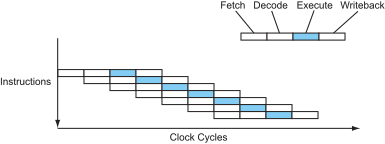
\includegraphics[width=0.7\textwidth]{images/pipelined2}
	\caption{Przepływ wykonywania instrukcji przez procesor potokowy \cite{ModernMicroprocessors90MinGuide}.}
\end{figure}

W takiej sytuacji procesor kończy wykonywać jedną instrukcję na cykl (w procesorze sekwencyjnym trwało to cztery cykle). Uzyskano zatem czterokrotne przyspieszenie, nie zmieniając taktowania procesora.

\subsection{Superpotokowość -- zwiększenie liczby etapów potoków}

Z uwagi na to, że prędkość wykonywania wielu instrukcji jest limitowana między innymi przez czas najwolniejszego etapu w potoku, etap taki można podzielić na mniejsze. W ten sposób wykonywanie kolejnej instrukcji będzie mogło rozpocząć się szybciej. 
Co prawda, z~powodu podziału instrukcje mogą wykonywać się przez więcej cykli (większe opóźnienie), ale~procesor wciąż będzie kończył jedną instrukcję na~cykl (większa przepustowość), zatem wykona więcej instrukcji w~tym samym czasie.

\begin{figure}[!h]
	\centering
	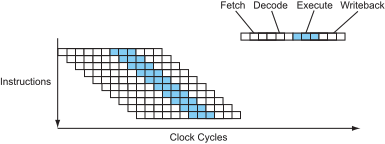
\includegraphics[width=0.7\textwidth]{images/superpipelined2}
	\caption{Przepływ wykonywania instrukcji przez procesor superpotokowy \cite{ModernMicroprocessors90MinGuide}.}
\end{figure}

\subsection{Superskalarność}

Kolejnym rozszerzeniem potoku jest zwiększenie liczby skalarnych jednostek wykonawczych. Dzięki temu taki superskalarny potok jest w stanie wykonywać kilka instrukcji jednocześnie.

\begin{figure}[!h]
	\centering
	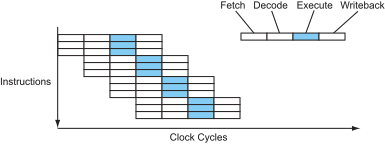
\includegraphics[width=0.7\textwidth]{images/superscalar2}
	\caption{Przepływ wykonywania instrukcji przez procesor superskalarny \cite{ModernMicroprocessors90MinGuide}.}
\end{figure}


\subsection{Superskalarność i superpotokowość}

Procesory mogą być także jednocześnie superskalarne i superpotokowe. Praktycznie wszystkie obecne procesory są projektowane w ten sposób. Zazwyczaj nazywa się je po prostu superskalarnymi, ponieważ superpotokowość to w rzeczywistości potokowość z większą liczbą etapów w potoku~\cite{ModernMicroprocessors90MinGuide}. 

\begin{figure}[!h]
	\centering
	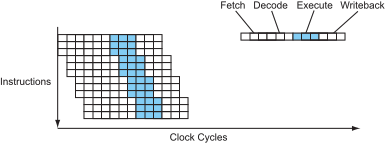
\includegraphics[width=0.7\textwidth]{images/superpipelinedsuperscalar2}
	\caption{Przepływ wykonywania instrukcji przez procesor superskalarny i superpotokowy~\cite{ModernMicroprocessors90MinGuide}.}
\end{figure}

\subsection{Zależności między instrukcjami}

Przetwarzanie potokowe musi sprostać wielu problemom. Jednym z takich problemów są zależności miedzy instrukcjami. Przykładowo:

\begin{lstlisting}[
    numbers=none,
    aboveskip={0.5\baselineskip},
]
a = b * 2;
d = a + e;
\end{lstlisting}

Druga instrukcja jest zależna od pierwszej, zatem nie można zacząć jej wykonywać do czasu, aż~zostanie zapisany wynik pierwszej.
W takim przypadku superskalarność nie zwiększy wydajności.


\subsection{Gałęzie wykonania (ang. \textit{branches})}
\label{sub:branches}
Kolejnym problemem dla potoku są instrukcje warunkowe. Przykładowo:

\begin{lstlisting}[
    numbers=none,
    aboveskip={0.5\baselineskip},
]
if (a == 3)
    b = c;
else
    b = d;
\end{lstlisting}
Co po przetłumaczeniu na instrukcje asemblera będzie wyglądać mniej więcej tak:
\begin{lstlisting}[
    numbers=none,
    aboveskip={0.5\baselineskip},
    language={[x86masm]Assembler}
]
	cmp a, 3  ; a == 3 ?
	jne L1	  ; skocz do L1, jeśli porównanie zwróciło fałsz
	mov c, b  ; przypisz b = c
	jmp L2	  ; skocz do L2
L1:	mov d, b  ; przypisz b = d
L2:	...
\end{lstlisting}

Aby nie marnować cennych cykli, procesory posiadają specjalną jednostkę odpowiedzialną za dynamiczną predykcję gałęzi (ang. \textit{dynamic branch prediction}). Jej działanie polega na tym, że procesor próbuje przewidzieć --~poprzez zapamiętywanie informacji w trakcie działania programu --~która z gałęzi powinna zostać wykonana, i tę zaczyna wykonywać.

Wynik instrukcji danej gałęzi nie zostaje zapisany do czasu wykonania się instrukcji warunkowej. Wtedy okazuje się, czy procesorowi udało się przewidzieć i kontynuuje pracę, czy~musi na~chwilę ją~przerwać i~usunąć z potoku wszystkie instrukcje, które pochodziły ze źle przewidzianej gałęzi. Następnie wykonuje on instrukcje poprawnej gałęzi.

Pracę procesora może także wspomóc programista (a~w~zasadzie kompilator) poprzez tak zwane statyczne przewidywanie gałęzi (ang. \textit{static branch prediction}). Kompilator może oznaczyć daną gałąź jako tą, którą program wykonuje częściej. Nowoczesne kompilatory (np. gcc czy~clang) pozwalają skompilować program tak, żeby podczas jego działania zapisywane były informacje, które z gałęzi zostały wykonane częściej\footnote{Taka optymalizacja to z ang. \textit{PGO -- profile guided optimization} -- czyli optymalizacja opierająca się na profilowaniu aplikacji.}. Następnie takie dane można wykorzystać podczas kolejnej kompilacji programu.


Istnieją także instrukcje, które eliminują gałęzie. Wcześniejszy przykład można zapisać tak:

\begin{lstlisting}[
    numbers=none,
    aboveskip={0.5\baselineskip},
    language={[x86masm]Assembler},
    morekeywords={cmovne}
]
	cmp 	a, 3  ; a == 3 ?
	mov 	c, b  ; przypisz b = c
	cmovne 	d, b  ; przypisz b = d, jeżeli ostatnie
	    	      ; porównanie jest fałszem
\end{lstlisting}

Wprowadzono tutaj nową instrukcję \texttt{cmovne} (ang. \textit{conditional move if not equal}). Instrukcja ta~zapisuje swój wynik tylko wtedy, gdy~warunek jest spełniony -- w~tym przypadku, jeżeli flaga ZF (ang.~\textit{zero flag}) w~rejestrze stanu jest nieustawiona (jest ona ustawiana przez instrukcję \texttt{cmp}, gdy wartości są~równe).

Zastosowanie nowej instrukcji z jednej strony skróciło kod, a z drugiej wyeliminowało problematyczne zjawisko predykcji gałęzi, które mogłoby spowodować zmarnowanie cykli procesora.

Wykorzystanie takiej instrukcji nie zawsze jest optymalizacją. W przypadku, gdy dana gałąź wykonania jest przewidywalna dla procesora, lepiej jest skorzystać z instrukcji skoku warunkowego. Jest tak ponieważ instrukcja przypisania warunkowego wprowadza więcej zależności między danymi.

\section{Jednoczesna wielowątkowość}

Jeżeli podczas wykonywania potoku procesor nie może wykonać kilku instrukcji niezależnie (na~przykład ze~względu na~zależności między nimi), to~potencjalnym źródłem instrukcji niezależnych mogą być inne wątki w~tym samym programie lub inne programy. Jednoczesna wielowątkowość (ang.~\textit{SMT --~Simultaneous multithreading}) jest techniką projektowania procesorów, która wykorzystuje taki typ zrównoleglania na~poziomie wątków.

Idea ta~polega na tym, żeby zastąpić ,,puste'' etapy w~potoku (na~przykład czekające na~wykonanie zależnej instrukcji) instrukcjami pochodzącymi z~innych wątków wykonujących się w~tym samym czasie, na~tym samym rdzeniu procesora. Procesor korzystający z~tej techniki w rzeczywistości korzysta z jednego fizycznego rdzenia. Z~poziomu systemu operacyjnego prezentuje się on~jako dwa lub więcej logiczne procesory.

Technika taka jest dużo wydajniejsza od~wielordzeniowego procesora pod względem wykorzystania przestrzeni układu elektronicznego, kosztu wykonania, zużycia energii czy~rozpraszania ciepła.

Implementacja SMT wymaga powielenia niewielkiej części komponentów procesora -- między innymi rejestrów procesora oraz tablicy TLB (ang. \textit{Translation Lookaside Buffer}) mapującej adresy pamięci wirtualnej na~adresy fizyczne. Większe i bardziej złożone komponenty, takie jak pamięć podręczna (ang. \textit{cache}), czy~jednostki wykonania (ang. \textit{execution units} czy~\textit{functional units})~są~współdzielone między wątkami jednego rdzenia.

Takie rozwiązanie pozwala na~ogólne zwiększenie wydajności procesora poprzez relatywnie mały wzrost kosztów produkcji jednego rdzenia.


\begin{figure}[!h]
	\centering
	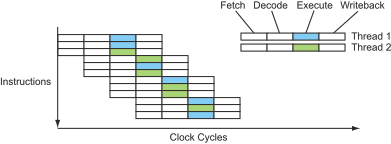
\includegraphics[width=0.7\textwidth]{images/smt2}
	\caption{Przepływ wykonywania instrukcji przez procesor wykorzystujący SMT \cite{ModernMicroprocessors90MinGuide}.}
\end{figure}

Wadą technologii SMT jest fakt, że~może ona zmniejszyć wydajność przetwarzania poprzez zmniejszenie ilości zasobów dostępnych dla wątku (pamięci podręcznej i tablicy TLB). Ze względu na~to~może się okazać, że~dany program bądź grupa programów będzie działać szybciej, gdy wyłączymy SMT.

Jedną z implementacji technologii SMT jest technologia firmy Intel zwana Hyper-Threading, która dzieli każdy z~rdzeni procesora na~dwa wątki. \cite{ModernMicroprocessors90MinGuide}


\section{Instrukcje wektorowe -- SIMD}
\label{sec:SIMD}

Nowoczesne procesory posiadają specjalne rozszerzenia, dodające nowe, duże rejestry oraz~instrukcje, pozwalające na wykonanie danej operacji na danych, znajdujących się w tych rejestrach (przykładowo, na zsumowanie czterech liczb z innymi czterema liczbami jednocześnie).

Instrukcje operujące na rejestrach zawierających kilka danych nazywa się instrukcjami wektorowymi i~określa się je~jako SIMD (ang. \textit{single instruction multiple data}).

W zależności od rozszerzenia, rejestry wektorowe mają różny rozmiar:

\begin{itemize}
    \item SSE (ang. \textit{Streaming SIMD Extensions}) -- 128 bit
    \item AVE (ang. \textit{Advanced Vector Extensions}) -- 256 bit
\end{itemize}

Rejestry te pozwalają na wykorzystanie różnych typów danych -- na przykład, w rejestrach XMM dodanych w rozszerzeniu SSE, można przechowywać:

\begin{itemize}
    \item 4 liczby typu float (32-bitowe liczby zmiennoprzecinkowe)
    \item 2 liczby typu double (64-bitowe liczby zmiennoprzecinkowe)
    \item 16 liczb typu int8 (8-bitowe liczby całkowite)
    \item 8 liczb typu int16 (16-bitowe liczby całkowite)
    \item 4 liczby typu int32 (32-bitowe liczby całkowite)
    \item 2 liczby typu int64 (64-bitowe liczby całkowite)
    \item jedną 	liczbę typu int128 (128-bitowa liczba całkowita)
\end{itemize}

Wykorzystanie instrukcji wektorowych pozwala na uzyskanie dużego przyspieszenia. 
Kompilatory z~najbardziej agresywną optymalizacją potrafią czasami zamienić kod posiadający rozgałęzienia --~które potrafią być kłopotliwe z~perspektywy wydajności --~na~taki, który ich nie~ma~oraz wykorzystuje instrukcje wektorowe. Przykład takiej optymalizacji został przedstawiony w~przykładzie opisanym w sekcji \ref{sub:filteredSum}.

\section{Problem dostępu do pamięci}

Około jedna czwarta instrukcji wykonywanych przez procesor to~ładowanie danych z pamięci. Aby~procesor mógł wydajnie działać, przesyłanie danych musi być dostatecznie szybkie.

Obecnie procesory są dużo bardziej skomplikowane niż 35 lat temu. W~tamtych czasach taktowanie procesorów wynosiło tyle, co~taktowanie szyny pamięci. W~konsekwencji dostęp do~pamięci był niewiele wolniejszy od~dostępu do~rejestrów procesora. Ta~tendencja zmieniła się we~wczesnych latach 90., kiedy to~zwiększano taktowanie procesora. Taktowanie szyny pamięci oraz wydajność kości RAM\footnote{ang. Random Access Memory – pamięć o~dostępie swobodnym} nie rosły proporcjonalnie do~prędkości procesora \cite{WhatEveryScientistShouldKnowAboutMemory}, co~przedstawia rysunek \ref{fig:cpu_mem_gap}.

\begin{figure}[!h]
	\centering
	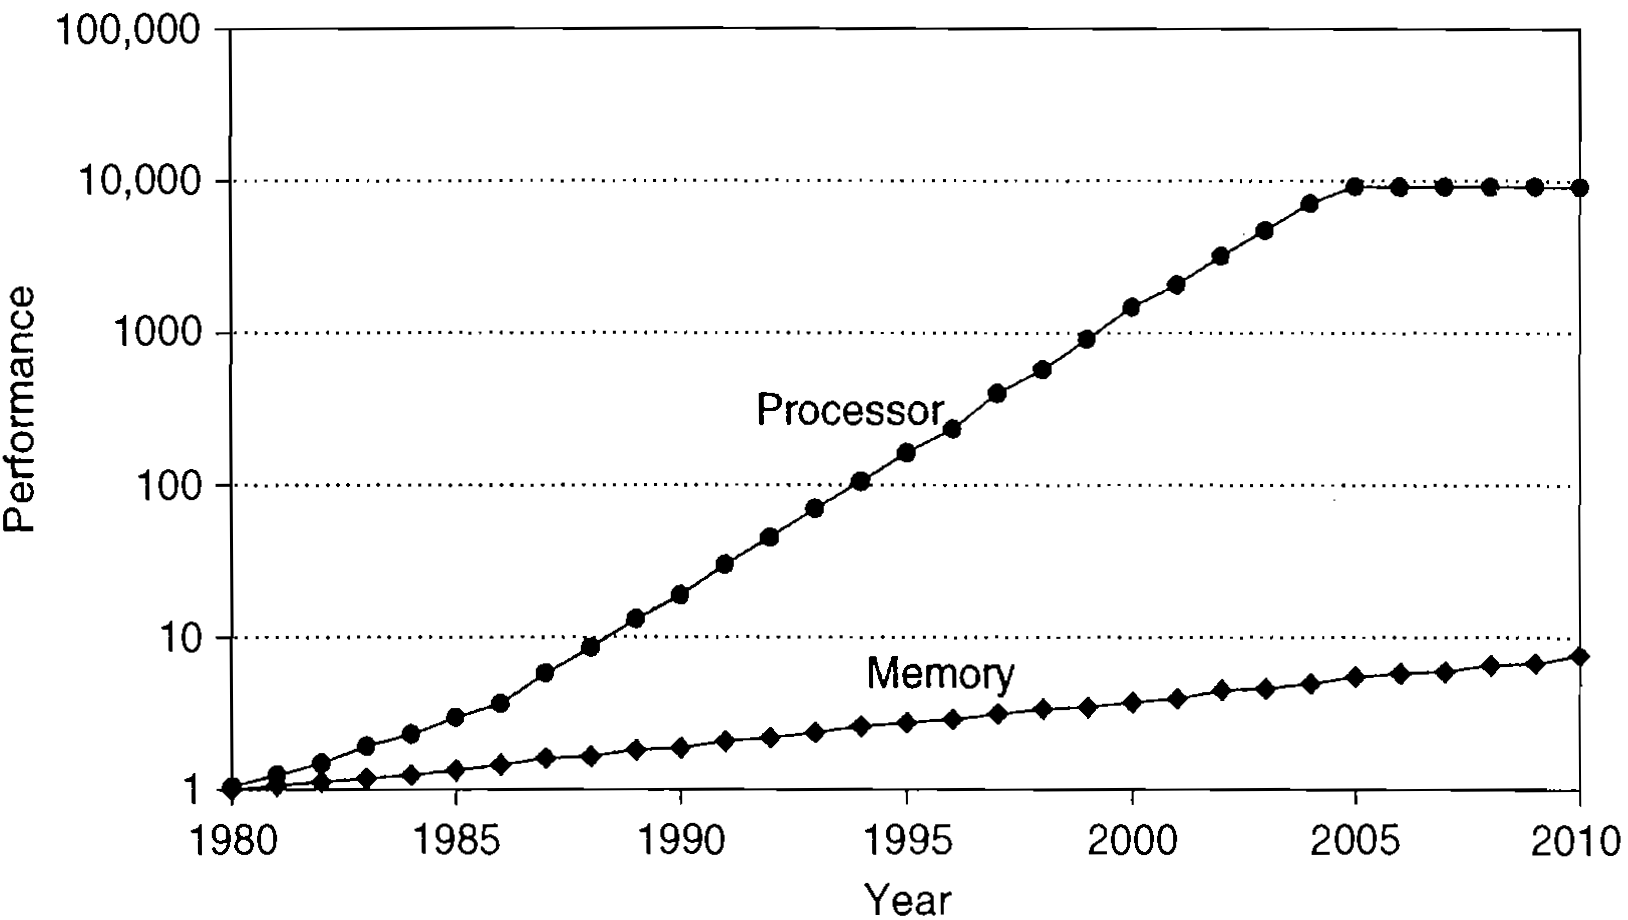
\includegraphics[width=0.65\textwidth]{images/cpu_to_memory_gap}
	\caption{Wykres przedstawia lukę w~wydajności na~przestrzeni lat, mierzoną jako różnica w~czasie pomiędzy odwołaniem do~pamięci przez procesor (pojedynczy procesor lub rdzeń) a~opóźnieniem w~dostępie do~pamięci DRAM, przy przyjęciu osiągów z~roku 1980 jako podstawy~\cite{cpu_mem_gap}.}
	\label{fig:cpu_mem_gap}
\end{figure}

Ze względu na~powyższe stworzono pamięć podręczną procesora (ang. \textit{cache}), do~której ładowane są~najczęściej wykorzystywane dane. Dostęp do~takiej pamięci jest dużo szybszy od~dostępu do~RAM-u. Wynika to~z~dwóch faktów -- po~pierwsze, jest ona wykonana w~technologii SRAM\footnote{SRAM -- ang. Static Random Access Memory -- statyczna pamięć o dostępie swobodnym}, w~przeciwieństwie do pamięci RAM, która jest pamięcią DRAM\footnote{DRAM -- ang. Dynamic Random Access Memory - rodzaj ulotnej pamięci półprzewodnikowej}. Po~drugie, fizycznie znajduje się bliżej procesora niż RAM, więc dane muszą zostać przesłane na~krótszą odległość.


\subsection{Hierarchia pamięci}

W komputerach osobistych wyróżniamy następującą hierarchię pamięci (od~najszybszej do~najwolniejszej):

\begin{itemize}
	\item rejestry procesora -- znajdują się wewnątrz każdego rdzenia procesora; to~na~nich procesor wykonuje obliczenia,
	\item pamięć podręczna procesora -- może być jej kilka poziomów,
	\item pamięć RAM,
	\item pamięć zewnętrzna SSD/HDD.
\end{itemize}

W tej pracy skupiono uwagę głównie na pamięci podręcznej procesora, bo~uwzględniając fakt jej istnienia i~to, jak działa, programiści są w~stanie pisać szybsze programy.

\subsection{Pamięć podręczna procesora}

Pamięć podręczna nie jest bezpośrednio dostępna dla programisty czy~dla systemu operacyjnego, a~zamiast tego całkowicie zarządza nią procesor. Jest ona wykorzystywana do~tworzenia tymczasowych kopii danych, które prawdopodobnie będą używane w~niedługim czasie przez procesor.

Proste obliczenia pozwalają wykazać, jak w~teorii efektywna może być pamięć podręczna.
Na~potrzeby przykładu można założyć, że dostęp do głównej pamięci zajmuje 200 cykli procesora, a~dostęp do~pamięci podręcznej -- 15 cykli. Wtedy kod, który używa 100 elementów, każdy po~100 razy, spędzi 2 000 000 cykli na~dostępie do~pamięci, gdy pamięć podręczna nie jest dostępna, a~tylko 168 500 cykli, gdy pamięć podręczna pomieści wszystkie dane. Fakt posiadania pamięci podręcznej zredukował ilość cykli o 91.5\% \cite{WhatEveryScientistShouldKnowAboutMemory}.

\subsection{Poziomy pamięci podręcznej}

Obecnie procesory nie pobierają danych bezpośrednio z RAM-u. Zamiast tego, pobierają je~z~wbudowanej pamięci podręcznej. W~zależności od procesora, ilość i~rozmiar pamięci podręcznych może się różnić; obecnie są~to~najczęściej trzy poziomy pamięci podręcznej -- L1, L2, L3. Procesor pobiera dane z~pamięci podręcznej L1, która pobiera je~z~L2, a~ta~z~kolei z~L3. Dane do~L3 pobierane są~bezpośrednio z~pamięci RAM.

Wielopoziomowa pamięć podręczna wynika z faktu, że im bliżej procesora fizycznie znajduje się pamięć podręczna oraz im mniejszy ma rozmiar, tym jest szybsza\footnote{Szerzej opisane w sekcji \ref{sub:CacheImpl}}. Pamięć podręczna pierwszego poziomu -- L1 zazwyczaj ma rozmiar 8-64 kB oraz dzieli się na L1d (ang. \textit{L1 data cache} --~pamięć podręczna danych) oraz L1i (ang. \textit{L1 instruction cache} -- pamięć podręczna instrukcji). Fizycznie znajduje się ona wewnątrz każdego rdzenia.
L2 przechowuje od kilkuset kilobajtów do kilku megabajtów danych i tak samo jak w przypadku L1, każdy rdzeń procesora posiada swoją pamięć L2.
L3 natomiast ma rozmiar kilku do kilkudziesięciu megabajtów. W~przeciwieństwie do L1 oraz L2, pamięć ta jest współdzielona między rdzeniami.

Transfer danych pomiędzy poziomami pamięci podręcznej oraz pamięcią RAM odbywa się w blokach o stałym rozmiarze -- najczęściej 32 lub 64 bajty, nazywanych liniami cache (ang. \textit{cache line}). Dzieje się tak dlatego, aby sprawdzenie, czy potrzebne dane znajdują się w pamięci podręcznej, nie było zbyt kosztowne  \cite{ModernMicroprocessors90MinGuide}.

Przykładowe hierarchie pamięci w nowoczesnych procesorach zostały przedstawione w~tabelach~\ref{tab:CoreI4Memory} oraz \ref{tab:AppleA8Memory}.

\clearpage

\begin{table}[!h]
	\centering
    \caption{Hierarchia pamięci w~procesorach Core i*4 Haswell \cite{ModernMicroprocessors90MinGuide}.}
    \label{tab:CoreI4Memory}
	\begin{tabular}{|2|c|c|7|}
		\hline
		Rodzaj pamięci & Rozmiar & Opóźnienie [cykle] &  Lokalizacja fizyczna \\
		\hline \hline
		L1 cache & 32 KB & 4 & wewnątrz każdego rdzenia \\
		\hline
		L2 cache & 256 KB & 11 & obok każdego rdzenia \\
		\hline
		L3 cache & 6 MB & ~21 & współdzielone między wszystkimi rdzeniami \\
		\hline
		L4 E-cache & 128 MB & ~58 & oddzielny układ eDRAM \\
		\hline
		RAM & 4+ GB & ~117 & kości SDRAM DIMM na płycie głównej \\
		\hline
		Swap & 100+ GB & 10000+ & dysk HDD lub SSD \\
		\hline
	\end{tabular}
\end{table}

\begin{table}[!h]
	\centering
    \caption{Hierarchia pamięci w~procesorach Apple A8 w~IPhone 6 \cite{ModernMicroprocessors90MinGuide}.}
    \label{tab:AppleA8Memory}
	\begin{tabular}{|2|c|c|7|}
		\hline
		Rodzaj pamięci & Rozmiar & Opóźnienie [cykle] &  Lokalizacja fizyczna \\
		\hline \hline
		L1 cache & 64 KB & 4 & wewnątrz każdego rdzenia \\
		\hline
		L2 cache & 1 MB & ~20 & obok dwóch rdzeni \\
		\hline
		L3 cache & 4 MB & ~107 & obok kontrolera pamięci \\
		\hline
		RAM & 1 GB & ~261 & kość SDRAM \\
		\hline
		Swap & N/A & N/A & stronicowanie oraz swapowanie nie są wykorzystywane przez iOS \\
		\hline
	\end{tabular}
\end{table}

Efektywność pamięci podręcznej wynika stąd, że pisząc odpowiednio aplikację, dostęp do~pamięci zajmie tylko kilka cykli zamiast kilkuset. Jest to~możliwe dzięki temu, że~w~wielu programach~zarówno kod programu, jak i~dane są~lokalne przestrzennie (ang. \textit{spatial locality}) oraz~czasowo (ang. \textit{temporal locality}) \cite{WhatEveryScientistShouldKnowAboutMemory, TheLocalityPrinciple}:

\begin{itemize}
	\item Lokalność przestrzenna -- podczas korzystania z danej komórki pamięci występuje duże prawdopodobieństwo, że program będzie odwoływał się do pamięci o bliskiej adresacji względem poprzednich danych (na przykład iteracja po tablicy).
	
	\item Lokalność czasowa -- podczas korzystania z danej komórki pamięci występuje duże prawdopodobieństwo, że program w krótkim czasie ponownie odwoła się do tych samych danych.
\end{itemize}


\subsection{Implementacja pamięci podręcznej}
\label{sub:CacheImpl}

Z punktu widzenia sprzętu pamięć podręczna stanowi kilka dwukolumnowych tabel. W~pierwszej kolumnie przechowywane są tagi służące do~adresowania, a~w drugiej dane. Kolejne wiersze są kolejnymi liniami cache. Tag to górna część adresu danych, które szukane są w~pamięci podręcznej. Dolna część adresu jest wykorzystywana jako indeks w~tabelach pamięci podręcznej.

Sprawdzenie, czy dany adres znajduje się w~pamięci podręcznej, to~w~praktyce porównanie, czy~na~danym indeksie w którejś z~tabel znajduje się dany tag. Przykład tego został przedstawiony na~rysunku~\ref{fig:cacheFetch}.

\begin{figure}[!h]
	\centering
	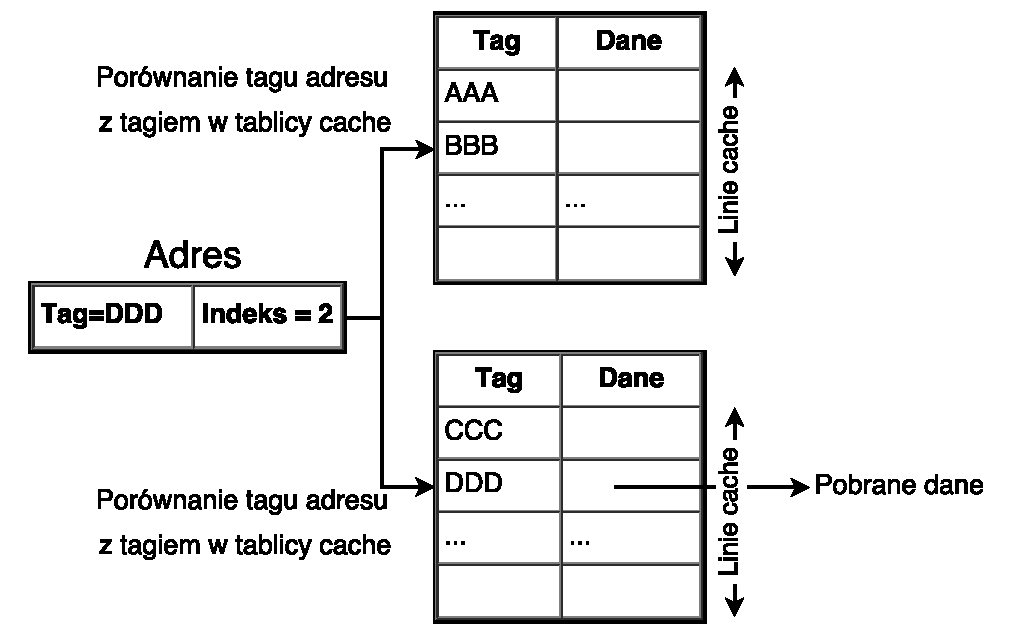
\includegraphics[width=0.7\textwidth]{images/cache_fetch}
	\caption{Sprawdzenie, czy dane znajdują się~w~pamięci podręcznej posiadającej dwie tablice.}
    \label{fig:cacheFetch}
\end{figure}

Sytuacja znalezienia danych w pamięci podręcznej nazywana jest trafieniem (ang. \textit{hit}) -- wtedy to~odpowiednie komórki przesyłane są do procesora. W przeciwnym razie dane wyszukiwane są w wyższych poziomach pamięci podręcznej lub pobierane z RAM-u. Sytuację nieznalezienia danych w cache nazywa~się chybieniem (ang. \textit{miss}) i powoduje ona utratę wydajności procesora, ponieważ musi on poczekać na dane.

\subsection{Asocjacyjność}
\label{cha:Associativity}

Jak można wywnioskować z rysunku \ref{fig:cacheFetch} pamięć podręczna nie przechowuje stricte najczęściej używanych danych, gdyż oznaczałoby to, że dane o dowolnych adresach można przechowywać w~dowolnych liniach cache. Z perspektywy zasad lokalności takie rozwiązanie byłoby bardzo korzystne. Niestety, oznaczałoby to~też utratę szybkiego dostępu do pamięci podręcznej, ze~względu na~potrzebę sprawdzenia wszystkich linii cache, czy dana komórka pamięci się w~danej linii znajduje.

Zamiast tego, dany adres w pamięci może znajdować się w jednej z kilku linii cache. Implementuje się to w ten sposób, że pamięć podręczną danego poziomu dzieli się na kilka tablic. Dzięki temu sprawdzenie, czy dany adres znajduje się w cache polega na wykonaniu tylu porównań, ile jest tych tablic. Sytuacja taka została przedstawiona na rysunku \ref{fig:cacheFetch}.

Pamięć podręczną zaprojektowaną w ten sposób nazywa się pamięcią zbiorowo-skojarzeniową (inaczej zbiorowo-asocjacyjną -- ang. \textit{set-associative cache}). Nazwa pochodzi stąd, że sprawdzenie, czy dany adres znajduje się w pamięci, działa poprzez skojarzenie -- to znaczy, każdy adres w pamięci RAM jest skojarzony ze zbiorem lokacji (linii cache) w pamięci podręcznej.

Z tego powodu, gdy wiele komórek pamięci mapuje się do tego samego indeksu, naprzemienny dostęp do nich będzie wolny, ponieważ procesor będzie ładował je naprzemiennie do pamięci podręcznej z pamięci podręcznej wyższego poziomu lub z RAM-u. Taką sytuację nazywamy konfliktem (ang. \textit{cache conflict}) lub~też zaśmiecaniem (ang. \textit{thrashing}) -- ponieważ, pomimo wykorzystywania tych samych danych, główne założenia pamięci podrecznej nie przynoszą korzyści.

Rozwiązaniem tego problemu jest po części zwiększenie ilości tablic pamięci podręcznej. W~ten sposób można ograniczyć efekt zaśmiecania kosztem utraty wydajności związanej z~równoległym sprawdzaniem, czy dane znajdują się w którejś z kilku tablic.

W nowoczesnych procesorach pamięć podręczna instrukcji zazwyczaj jest w dużym stopniu skojarzeniowa, ponieważ opóźnienie, które wynika z dodatkowej logiki na równoległe sprawdzenie wielu tablic, jest ukryte przez pobieranie i buforowanie we wczesnych etapach potoku procesora.

Z drugiej strony, pamięć podręczna danych jest w~mniejszym stopniu skojarzeniowa, aby~zminimalizować opóźnienie związane z~ładowaniem danych (które było istotnym powodem stworzenia pamięci podręcznej).

Większość procesorów posiada cztery tablice w~zbiorowo-skojarzeniowej pamięci podręcznej, ale~istnieją też~takie, które posiadają dwie (na przykład Athlon, Athlon 64/Phenom, PowerPC G5 oraz Cortex-A15/A57). Są~też~takie, które posiadają ich 8 -- PowerPC G4e, Pentium~M oraz~jego wielordzeniowi następcy.

Ostatnia ,,deska ratunku'' przed odwołaniem się do pamięci RAM, czyli duża pamięć podręczna L2 lub L3, jest zazwyczaj także wysoko skojarzeniowa -- zawiera 12 lub 16 tablic \cite{ModernMicroprocessors90MinGuide}.


\subsection{Tagi w pamięci cache}

Projektując pamięć podręczną, jako tag można wykorzystać adresy pamięci fizycznej albo~wirtualnej (opisanej w sekcji \ref{sec:VirtualMemory}).

W przypadku wykorzystania adresów pamięci wirtualnej, problem będzie sprawiał fakt, że~różne programy mogą używać tych samych adresów pamięci wirtualnej do mapowania innych adresów fizycznych. Aby to naprawić, pamięć podręczna musi zostać wyczyszczona (ang.~\textit{flushed}) podczas każdej zmiany kontekstu (ang.~\textit{context switch})\footnote{Zmiana kontekstu to~proces polegający na zapisie stanu danego procesu lub~wątku i odczycie zapisanego stanu kolejnego. Dzięki temu wykonanie procesu lub~wątku może zostać później wznowione z miejsca, w~którym został on zatrzymany. W~taki sposób wiele procesów może wykonywać się ,,równolegle'' na~jednym procesorze. Taką funkcjonalnością cechują się wielozadaniowe systemy operacyjne. \cite{ContextSwitching}}.

Z drugiej strony, użycie adresów fizycznych jako tagów oznacza, że podczas sprawdzania, czy~adres znajduje się w~pamięci podręcznej, należy przeprowadzić translację adresu wirtualnego na fizyczny. Taka operacja spowalnia ów test.

Powszechnym sposobem jest zastosowanie adresów wirtualnych do indeksowania pamięci podręcznej oraz adresów fizycznych jako tagów. Mapowanie adresów wirtualnych na fizyczne --~poprzez mechanizm \textit{TLB lookup} (ang.) -- może być wtedy wykonane równolegle z~wyciągnięciem tagu o~podanym indeksie z~pamięci podręcznej, dzięki czemu będzie on szybciej dostępny i~porównany z~tagiem. Takie rozwiązanie nazywa się wirtualnie indeksowaną, fizycznie tagowaną pamięcią podręczną (ang. \textit{virtually-indexed physically-tagged cache}) \cite{ModernMicroprocessors90MinGuide}.

\section{Pamięć wirtualna}
\label{sec:VirtualMemory}
Pamięć wirtualna jest mechanizmem zarządzania pamięcią, dostępnym we współczesnych systemach operacyjnych ogólnego przeznaczenia, który daje procesom wrażenie pracy w ciągłej przestrzeni adresowej. Polega on na mapowaniu adresów pamięci używanych przez proces, nazywanych adresami wirtualnymi, na adresy fizyczne w RAM-ie lub w pamięci zewnętrznej.

Dzięki temu rozwiązaniu, program działający w systemie widzi pamięć operacyjną, jakby w całości należała do niego. Jest w ten sposób odizolowany od innych procesów i nie może modyfikować należących do nich obszarów pamięci \footnote{Oczywiście systemy operacyjne dostarczają specjalny mechanizm pamięci współdzielonej, dzięki której procesy mogą się ze sobą komunikować.}. Ułatwia to znacząco pisanie programów, gdyż programiści nie muszą dbać o to, czy odwołują się do pamięci zajmowanej przez inne procesy, czy nie.

Wirtualna przestrzeń adresowa jest implementowana zarówno sprzętowo, jak~i~programowo -- w procesorze znajduje się specjalna jednostka zarządzania pamięcią (\textit{ang. MMU -- Memory Management Unit}), która przeprowadza translację z adresów pamięci wirtualnej na~adresy pamięci fizycznej, a~system operacyjny odpowiada za~wypełnianie tabelę tzw. stron pamięci.

%Adresy wirtualne są 32-bitowymi wartościami na 32-bitowych systemach, a~64-bitowymi na~64-bitowych. 

W~rzeczywistości procesory mapują adresy ,,stron'' pamięci, czyli bloków o~konkretnym rozmiarze. Typowym rozmiarem strony w~systemach 32-bitowych, jak i 64-bitowych jest 4 kB. Wartość tę~da~się zmienić -- przykładowo, w~systemach opartych na~jądrze Linux, wymaga to~rekompilacji jądra systemu.

Aby każde odwołanie do zmiennej w programie nie wymagało translacji adresu wirtualnego na fizyczny, przetłumaczone adresy stron zapisywane są w specjalnej pamięci podręcznej TLB~(ang. \textit{translation lookaside buffer}) \cite{WhatEveryScientistShouldKnowAboutMemory}.

\section{Wczesne pobieranie}

Wczesne pobieranie (ang. \textit{prefetching}) jest techniką ,,ukrywania'' opóźnień związanych z~dostępem do~pamięci. Polega ono na~tym, że~dane pobierane są~z~pamięci na~krótko przed tym, gdy procesor ich faktycznie potrzebuje. Wyróżniamy dwa rodzaje wczesnego pobierania:

\begin{itemize}
	\item Sprzętowe -- procesory posiadają specjalne układy, które monitorując schematy dostępu do~danych, przewidują, które dane kolejno będą używane i~pobierają je~do~procesora. Proces ten jest automatyczny, programista nie~ma~na~niego bezpośredniego wpływu. Układy takie nazywane są~jednostkami wczesnego pobierania (ang.~\textit{prefetcher}).
	
	\item Programowe -- procesory posiadają specjalne instrukcje, informujące procesor, że~pamięć o~danym adresie będzie niedługo potrzebna --~wadą tego podejścia jest narzut na~wykonanie instrukcji.
\end{itemize}

Większość dzisiejszych procesorów posiada kilka układów wczesnego pobierania -- na przykład procesory firmy Intel z rodzin  Nehalem, Westmere, Sandy Bridge, Ivy Bridge, Haswell oraz Broadwell posiadają ich cztery -- dwa dla pamięci podręcznej pierwszego poziomu oraz dwa dla drugiego poziomu \cite{IntelHWPrefetchDisclosure, IntelOptimizationRefManual}.

\section{Języki programowania a ułożenie danych}
\label{cha:programming_langs}

Poniżej przedstawiono kilka faktów na temat możliwości ułożenia danych w kilku najpopularniejszych językach programowania według indeksu Tiobe z grudnia 2015 \cite{TiobeIndex}.

\begin{itemize}
	
	\item Python, PHP, Perl, Ruby, JavaScript -- jako języki interpretowane, czyli programy działające jak~maszyny wirtualne, nie dają wielu możliwości. Niektóre z~nich mają mechanizmy pozwalające na~przykład zmniejszyć ilość pamięci zajmowanej przez obiekty zdefiniowanego typu (np.~mechanizm \texttt{\_\_slots\_\_} w~języku Python \cite{PythonSlots}).
	
	\item Java, C\#, Visual Basic .NET -- programy w tych językach są~uruchamiane wewnątrz maszyny wirtualnej oraz posiadają mechanizm automatycznego zarządzania pamięcią. Z~perspektywy tworzenia kolekcji obiektów, nie ma pewności, czy będą one ułożone kolejno w pamięci. Co~ciekawe, jednym z~etapów mechanizmu odśmiecania (ang. \textit{garbage collector}) jest kompaktowanie obiektów --~czyli przemieszczanie ich w~celu defragmentacji pamięci~\cite{JavaCompacting, CSharpCompacting}\footnote{W~przypadku języka C\# istnieje różnica między strukturami oraz klasami -- instancje struktur są~tworzone na~stosie. Elementy tablicy struktur będą ułożone w~ciągłym obszarze pamięci. Zarówno w~Javie, jak~i~w~C\# tablica obiektów klas przechowuje w~ciągłym obszarze pamięci referencje (wskaźniki) do~właściwych elementów. Te mogą być dowolnie ulokowane w~pamięci. Osoby zaangażowane w~rozwój języka Java chcą tę~sytuację poprawić i stworzyć tzw. \textit{value objects} (ang.)~\cite{JavaValueObjects}, które są odpowiednikiem struktur w~C\#.}.
	
	\item C, C++ -- dzięki bezpośredniej możliwości operowania na wskaźnikach oraz braku jakiejkolwiek maszyny wirtualnej, programista ma największy wpływ na~ułożenie danych w~pamięci.

\end{itemize}

\section{Wyrównanie danych}
\label{cha:DataAlignment}

Wyrównanie danych to sposób ułożenia oraz dostępu do danych w pamięci. Zmienna jest ,,naturalnie wyrównana'', jeśli znajduje się pod adresem, który jest wielokrotnością jej rozmiaru. Dla przykładu: \mbox{32-bitowa} zmienna jest naturalnie wyrównana, jeżeli znajduje się pod adresem, który jest wielokrotnością 4 (ponieważ 32 bity to 4 bajty).

Procesory oparte o~niektóre architektury (np. bazujące na~architekturach Alpha, IA-64, MIPS oraz~SuperH) nie pozwalają na~odczyt niewyrównanych danych. Inne zaś zezwalają na~taki dostęp, często tracąc przy tym na~wydajności \cite{RefusingUnalignedAccessArchitectures}.

Kompilatory języków takich jak C czy C++ wyrównują dane w~sposób przedstawiony w~tabeli \ref{tab:CDataAlignment}.

\begin{table}[!h]
	\centering
    \caption{Typowe wyrównanie danych na 32 oraz 64 bitowych procesorach na systemie Linux przez kompilator firmy Intel~\cite{IntelDataAlignment}.}
    \label{tab:CDataAlignment}
	\begin{tabular}{|c|4|4|}
		\hline
		Typ danych & Wyrównanie na procesorze 32-bit (w~bajtach) & Wyrównanie na procesorze 64-bit (w~bajtach) 
		\\ \hline \hline
		char & 1 & 1
		\\ \hline
		short & 2 & 2
		\\ \hline
		int & 4 & 4
		\\ \hline
		long & 8 & 8
		\\ \hline
		float & 4 & 4
		\\ \hline
		double & 8 & 8
		\\ \hline
		long long & 8 & 8
		\\ \hline
		long double & 4 & 16
		\\ \hline
		dowolny wskaźnik & 4 & 8
		\\ \hline
	\end{tabular}
\end{table}

\subsection{Wyrównanie danych w strukturach}

Gdy struktura przechowuje elementy różnych typów, kompilator wstawia nieużywaną pamięć pomiędzy nie, aby je wyrównać. Proces ten nazywany jest dopełnieniem (ang. \textit{padding}). Zwiększa on~wydajność dostępu do~danych kosztem zwiększenia używanej pamięci.

Dopełnienie może także wystąpić na~końcu struktury, w~celu wyrównania jej samej (dzieje się tak w~przykładzie zawartym w~listingach \ref{lst:PaddingExample}, \ref{lst:ClangPaddingExample} oraz \ref{lst:GccPaddingExample}) \cite{IntelDataAlignment}.

Aby poznać faktyczne ułożenie danych przez kompilator, można skorzystać z~odpowiedniej flagi kompilatora clang lub dodatku do debuggera gdb o~nazwie \href{https://github.com/PhilArmstrong/pahole-gdb}{pahole-gdb (dostęp w~dniu 2015-12-15)}. Istnieje także dedykowana aplikacja pahole, lecz nie wspiera ona standardu c++11.

W listingach \ref{lst:ClangPaddingExample} oraz \ref{lst:GccPaddingExample} przedstawiono ułożenie danych przez kompilator clang++-3.6  oraz~\mbox{g++-5.2.1} dla przykładu z listingu \ref{lst:PaddingExample}. Program został skompilowany na 64-bitowym systemie Ubuntu 15.10.

\clearpage % TODO / FIXME

\begin{lstlisting}[
    caption=Program z przykładową strukturą danych., label=lst:PaddingExample
]
struct S {
    int a;
    bool b;
    int* c;
    bool e;
    int f;
    bool g;
    int h;
    bool i;
};

int main() {
    // Poniżej wykorzystano obiekt struktury oraz jego rozmiar.
    // Instrukcje te są wymagane dla funkcjonalności wyświetlenia 
    // organizacji struktury przez clang oraz pahole-gdb.
    S s;
    return sizeof(S);
}
\end{lstlisting}


\begin{lstlisting}[
    numbers=none,
    aboveskip={0.5\baselineskip},
    language={bash},
    caption={Ułożenie danych oraz padding przez kompilator clang++-3.6. Pierwsza kolumna oznacza z ang. \textit{offset} -- przesunięcie względem początku struktury. Dodatkowe informacje o~strukturze prezentowane są na końcu\protect\footnotemark.}, 
    label=lst:ClangPaddingExample
]
$ clang++-3.6 -cc1 -fdump-record-layouts struct_S.cpp 

*** Dumping AST Record Layout
0  | struct S
0  |   int a
4  |   _Bool b
8  |   int * c
16 |   _Bool e
20 |   int f
24 |   _Bool g
28 |   int h
32 |   _Bool i
   | [sizeof=40, dsize=40, align=8
   |  nvsize=40, nvalign=8]
\end{lstlisting}

\footnotetext{Sizeof -- rozmiar struktury. Dsize -- rozmiar danych (bez dopełnienia na końcu struktury). Align -- wyrównanie obiektów struktury. Nvsize -- rozmiar struktury bez uwzględnienia wskaźnika na tablicę funkcji wirtualnych (jeśli struktura takowy posiada). Nvalign -- wypełnienie bez uwzględnienia wskaźnika na tablicę funkcji wirtualnych.}

\begin{lstlisting}[
    numbers=none,
    aboveskip={0.5\baselineskip},
    language={bash},
    keywords={},
    caption={Ułożenie danych oraz padding przez kompilator g++ 5.2.1.  Dodatek pahole-gdb w~przypadku linii zawierającej deklarację struktury wyświetla jej całkowity rozmiar. W przypadku linii zawierających pola, wyświetlane są dodatkowo przesunięcie względem początku struktury, rozmiar danego pola oraz -- jeżeli występuje -- informacja o rozmiarze ,,dziury'', czyli dopełnienia, aby następne pole było wyrównane.}, label=lst:GccPaddingExample
]   
$ g++ -std=c++11 -g struct_S.cpp -o exec
$ gdb --quiet ./exec
Reading symbols from ./exec...done.
(gdb) pahole S
/*   40     */ struct S {
/*   0    4 */    int a
/*   4    1 */    bool b
/* XXX 24 bit hole, try to pack */
/*   8    8 */    int * c
/*  16    1 */    bool e
/* XXX 24 bit hole, try to pack */
/*  20    4 */    int f
/*  24    1 */    bool g
/* XXX 24 bit hole, try to pack */
/*  28    4 */    int h
/*  32    1 */    bool i
} 
\end{lstlisting}

Jak można zaobserwować, oba kompilatory ułożyły dane tak samo. W obu przypadkach, na~dopełnienie trzech zmiennych typu \texttt{bool} zmarnowane zostały 72 bity.

Zmarnowane miejsce można zaoszczędzić, zmieniając kolejność pól w strukturze danych --~ustawiając je od największego rozmiaru pola do najmniejszego \footnote{Jest to generalna zasada. Są jednak przypadki, w których, pomimo nie zastosowania się do tej zasady, da~się uzyskać optymalny rozmiar struktury (zawierający najmniejsze możliwe dopełnienie lub jego brak).}.

Oszczędność miejsca w ten sposób zwiększa oczywiście wydajność -- przykładowo, w~przypadku wykorzystania tablicy struktur, więcej elementów zmieści się w jednej linii cache. Ułożenie takie zostało przedstawione w listingu \ref{lst:GoodPaddingExample} wraz z organizacją struktury -- dla kompilatora clang w listingu \ref{lst:ClangGoodPaddingExample} oraz~g++  w~listingu \ref{lst:GccGoodPaddingExample}.

\begin{lstlisting}[
    numbers=none,
    aboveskip={0.5\baselineskip},
    caption={Wydajniejsze ułożenie danych. Pola zostały rozlokowane od największego do najmniejszego rozmiaru.},
    label=lst:GoodPaddingExample
]
struct S {
	int* c;
	int a;
	int f;
	int h;
	bool b;
	bool e;
	bool g;
	bool i;
};
\end{lstlisting}


\begin{lstlisting}[
    numbers=none,
    aboveskip={0.5\baselineskip},
    language={bash},
    keywords={},
    caption={Ułożenie danych przez kompilator clang. Pola zostały rozlokowane od największego do najmniejszego rozmiaru.}, label=lst:ClangGoodPaddingExample
]
$ clang++-3.6 -cc1 -fdump-record-layouts struct_S_good.cpp 

*** Dumping AST Record Layout
0  | struct S
0  |   int * c
8  |   int a
12 |   int f
16 |   int h
20 |   _Bool b
21 |   _Bool e
22 |   _Bool g
23 |   _Bool i
   | [sizeof=24, dsize=24, align=8
   |  nvsize=24, nvalign=8]
\end{lstlisting}


\begin{lstlisting}[
    numbers=none,
    aboveskip={0.5\baselineskip},
    language={bash},
    keywords={},
    caption={Ułożenie danych przez kompilator g++. Pola zostały rozlokowane od największego do najmniejszego rozmiaru.},
    label=lst:GccGoodPaddingExample
]
$ g++ -std=c++11 -g struct_S_good.cpp -o exec
$ gdb --quiet ./exec
Reading symbols from ./exec...done.
(gdb) pahole S
/*   24     */ struct S {
/*   0    8 */    int * c
/*   8    4 */    int a
/*  12    4 */    int f
/*  16    4 */    int h
/*  20    1 */    bool b
/*  21    1 */    bool e
/*  22    1 */    bool g
/*  23    1 */    bool i
}
\end{lstlisting}

Tym razem w obu przypadkach struktura zajmuje 24 bajty i nie posiada żadnego dopełnienia.

\subsection{Zmiana wyrównania}

Istnieją uzasadnione przypadki, gdy należy zmienić wyrównanie struktury, bądź jej pól. Przykładem takim może być implementacja niskopoziomowych sterowników, gdy dane urządzenie wymaga odpowiedniej organizacji danych.

W ogólnym przypadku raczej się tego nie stosuje, ze względu na utratę wydajności, co zostało pokazane w rozdziale \ref{cha:DataAlignment}.

W kompilatorze Microsoft Visual C++, wyrównanie można zmienić poprzez dyrektywę preprocesora \texttt{\#pragma pack}, a w gcc oraz clang oprócz \texttt{\#pragma pack} można także wykorzystać specjalny atrybut \texttt{\_\_attribute\_\_((packed))}.

W listingach \ref{lst:PackedDataStructure}, \ref{lst:ClangPackedDataStructure} oraz \ref{lst:GccPackedDataStructure} pokazano organizację danych upakowanej struktury z listingu \ref{lst:PaddingExample}.

\begin{lstlisting}[
    aboveskip={0.5\baselineskip},
    caption={Upakowana struktura danych.},
    label=lst:PackedDataStructure
]
// ustawienie wyrównania do jednego bajtu
#pragma pack(1)
struct S {
    int a;
    bool b;
    int* c;
    bool e;
    int f;
    bool g;
    int h;
    bool i;
};
// przywrócenie domyślnego ustawienia wyrównania
#pragma pack()

int main() {
    S s;
    return sizeof(S);
}
\end{lstlisting}

\begin{lstlisting}[
    numbers=none,
    aboveskip={0.5\baselineskip},
    language={bash},
    keywords={},
    caption={Upakowana organizacja danych przez kompilator clang.},
    label=lst:ClangPackedDataStructure
]
$ clang++-3.6 -cc1 -fdump-record-layouts struct_S_packed.cpp

*** Dumping AST Record Layout
0  | struct S
0  |   int a
4  |   _Bool b
5  |   int * c
13 |   _Bool e
14 |   int f
18 |   _Bool g
19 |   int h
23 |   _Bool i
   | [sizeof=24, dsize=24, align=1
   |  nvsize=24, nvalign=1]
\end{lstlisting}
\clearpage %TODO
\begin{lstlisting}[
    numbers=none,
    aboveskip={0.5\baselineskip},
    language={bash},
    keywords={},
    caption={Upakowana organizacja danych przez kompilator g++.},
    label=lst:GccPackedDataStructure
]
$ g++ -g -std=c++11 struct_S_packed.cpp -o exec
$ gdb --quiet ./exec
Reading symbols from ./exec...done.
(gdb) pahole S
/*   24     */ struct S {
/*   0    4 */    int a
/*   4    1 */    bool b
/*   5    8 */    int * c
/*  13    1 */    bool e
/*  14    4 */    int f
/*  18    1 */    bool g
/*  19    4 */    int h
/*  23    1 */    bool i
}
\end{lstlisting}
